\documentclass[12pt,a4paper]{report}

% --- Essential Packages ---
\usepackage[utf8]{inputenc}
\setlength{\textwidth}{6.5in}
\setlength{\textheight}{9.0in}
\setlength{\oddsidemargin}{0in}
\setlength{\evensidemargin}{0in}
\setlength{\topmargin}{-0.5in}
\usepackage{setspace}
\onehalfspacing

% --- Math & Symbols ---
\usepackage{amsmath,amssymb,amsfonts}

% --- Graphics, Tables & PGFPlots ---
\usepackage{graphicx}
\usepackage{booktabs}
\usepackage{array}
\usepackage{tikz}
\usepackage{pgfplots}
\pgfplotsset{compat=1.18}

% --- Hyperlinks & Citations ---
\usepackage[numbers,sort&compress]{natbib}
\usepackage{hyperref}
\hypersetup{
	colorlinks=true,
	linkcolor=blue,
	citecolor=blue,
	urlcolor=blue
}

% --- Table of Contents Configuration ---
\setcounter{tocdepth}{2}

% --- Document Metadata ---
\title{
	\Huge \textbf{Uncertainty-Aware Multimodal Neural Networks for Explainable Skin Cancer Risk Stratification}\\[0.5em]
	\Large A Quantitative Evaluation of Explanation Faithfulness and Clinical Triage
}
\author{\textbf{Ameyaw Emmanuel Kakari}}
\date{\today}

\begin{document}
	
	\maketitle
	
	% --- Abstract ---
	\begin{abstract}
		The automated risk stratification of malignant skin lesions represents a critical juncture where artificial intelligence intersects with clinical decision support. While existing computer vision models achieve high diagnostic accuracy on standardized imagery, their clinical utility is limited by opaque decision boundaries, single-modality bias, and an inability to express epistemic uncertainty. This thesis presents a robust, multimodal neural architecture that fuses high-resolution 3D Total-Body Photography (TBP) lesion crop embeddings (via EfficientNet-B0) with structured clinical patient metadata (via Tabular MLP encoders) to predict lesion malignancy. Emphasizing clinical safety over raw accuracy, the system is optimized to maximize minority-class Sensitivity at a fixed Specificity threshold, accounting for the severe cost asymmetry between false positives and false negatives in skin cancer triage. 
		
		Beyond predictive performance, this research investigates the faithfulness of post-hoc explainability methods. We quantitatively evaluate visual attribution (Grad-CAM++) and tabular feature importance (KernelSHAP on input attributes) using Pixel Deletion/Insertion AUC and model weight randomization sanity checks, ensuring explanations track internal decision boundaries rather than inducing visual confirmation bias. Furthermore, we implement Monte Carlo (MC) Dropout to estimate epistemic uncertainty, enabling an automated triage mechanism that defers high-variance, ambiguous predictions to human expert review. Evaluated on a patient-stratified subset of the ISIC 2024 SLICE-3D dataset ($N=40,106$ lesions across $12,925$ unique patients) using strict patient-level cross-validation and an isolated holdout test set, our multimodal system demonstrates superior precision-recall characteristics compared to unimodal baselines, providing calibrated, faithful, and uncertainty-aware decision support.
	\end{abstract}
	
	% Add Abstract to Table of Contents
	\phantomsection
	\addcontentsline{toc}{chapter}{Abstract}
	
	\tableofcontents
	\newpage
	
	% --- Chapter 1 ---
	\chapter{Introduction}
	\label{ch:intro}
	
	\section{Clinical Context and Motivation}
	Skin cancer, particularly malignant melanoma and invasive carcinomas, poses a major global health challenge where early and accurate diagnosis directly correlates with patient survivability. Dermatologists routinely synthesize heterogeneous data modalities—combining visual inspection of lesion morphology with critical patient metadata such as age, biological sex, anatomical site, and lesion diameter. However, the majority of current deep learning diagnostic systems rely exclusively on pixel-level visual evidence \cite{esteva2017dermatologist}, artificially isolating the image from its broader clinical context. 
	
	Furthermore, the deployment of ``black-box'' neural networks in high-stakes medical domains has met justifiable resistance from clinical practitioners. A model that outputs a confident but incorrect benign diagnosis (a False Negative) carries catastrophic clinical consequences. To bridge the gap between algorithmic capability and clinical trust, an Explainable Artificial Intelligence (XAI) system must not only achieve high sensitivity but must also explicitly justify its predictions, quantify its own uncertainty, and recognize when it is operating under high epistemic ambiguity. 
	
	\section{Problem Statement}
	Despite advances in medical computer vision, three fundamental problems persist in automated skin lesion classification:
	\begin{enumerate}
		\item \textbf{Modality Isolation:} Models trained purely on images fail to leverage critical epidemiological priors (e.g., an identical visual lesion carries a vastly different risk profile on a 75-year-old male's scalp versus a 20-year-old female's torso).
		\item \textbf{Explanation Faithfulness:} Saliency maps and visual heatmaps frequently fail sanity checks, acting as sophisticated edge-detectors that look clinically plausible but do not faithfully represent the network's underlying decision boundaries \cite{adebayo2018sanity}.
		\item \textbf{Overconfidence in Ambiguity:} Standard softmax outputs are notoriously poorly calibrated and lack mechanisms to express epistemic uncertainty, leading to silent failures on ambiguous clinical presentations.
	\end{enumerate}
	
	\section{Research Questions}
	This research directly addresses these limitations through the following formal research questions:
	\begin{itemize}
		\item \textbf{RQ1 (Multimodal Synergy):} Does late-fusion of 3D total-body photography lesion crop representations with tabular clinical metadata yield a statistically significant improvement in minority-class Sensitivity ($\text{Recall} \ge 0.95$) and PR-AUC over unimodal baseline models on highly imbalanced datasets?
		\item \textbf{RQ2 (Explanation Faithfulness):} Do localized visual attributions (Grad-CAM++) and tabular attributions (KernelSHAP) satisfy quantitative algorithmic faithfulness criteria (measured via Pixel Deletion/Insertion AUC) and pass model weight randomization sanity checks?
		\item \textbf{RQ3 (Uncertainty-Gated Triage):} Can the integration of epistemic uncertainty estimation (via Monte Carlo Dropout variance, $\hat{\sigma}^2 > \tau$) successfully identify ambiguous inputs and defer them to expert review, thereby reducing the system's False Negative Rate (FNR) to $< 2\%$ while keeping human deferral volume clinically viable ($\le 15\%$)?
	\end{itemize}
	
	\section{Methodological Rigor and Bias Mitigation}
	A secondary but critical focus of this thesis is the adherence to strict methodological hygiene. Public lesion datasets (such as ISIC 2024 SLICE-3D) contain multiple image crops originating from individual patients. Naive image-level random splitting induces severe data leakage, as the network learns to recognize patient-specific background features (skin tone, lighting, hair patterns) rather than pathological structures, artificially inflating test metrics \cite{bisla2019towards}. This work employs rigorous \texttt{StratifiedGroupKFold} partitioning on \texttt{patient\_id} to guarantee zero patient overlap between training, validation, and holdout test folds. Additionally, the system evaluates demographic fairness by auditing subgroup-specific diagnostic performance across biological sex and age strata.
	
	\section{Summary of Contributions}
	The core contributions of this thesis are as follows:
	\begin{enumerate}
		\item The design and evaluation of a dual-branch late-fusion multimodal architecture (EfficientNet-B0 and Tabular MLP) optimized via focal loss for imbalanced clinical risk stratification.
		\item A quantitative evaluation pipeline for XAI algorithmic faithfulness, moving beyond qualitative visual inspection by implementing Pixel Deletion/Insertion curves and structural sanity checks.
		\item The formulation and integration of an uncertainty-aware clinical triage mechanism utilizing MC Dropout and Temperature Scaling to calibrate confidence and trigger automated expert referral.
		\item A fully reproducible, open-source codebase including a deployment-ready FastAPI backend and an interactive Streamlit clinical dashboard tailored for Research Clinical Decision Support (CDSS-R).
	\end{enumerate}
	
	\section{Thesis Structure}
	The remainder of this thesis is organized as follows: Chapter \ref{ch:related_work} reviews the state-of-the-art in multimodal medical deep learning, XAI, and uncertainty quantification. Chapter \ref{ch:methodology} details the mathematical formulations of the proposed architecture, data splitting protocols, and explainability evaluation metrics. Chapter \ref{ch:experiments} presents the experimental setup, baseline comparisons, and primary classification results on cross-validation and holdout test sets. Chapter \ref{ch:explainability} evaluates the algorithmic faithfulness of generated explanations and the efficacy of the uncertainty-gated triage system. Finally, Chapter \ref{ch:conclusion} discusses demographic fairness, clinical limitations, and directions for future research.
	
	% --- Chapter 2 ---
	\chapter{Related Work}
	\label{ch:related_work}
	
	\section{Computer Vision in Automated Skin Lesion Classification}
	Automated skin lesion diagnosis has advanced rapidly following the deployment of deep Convolutional Neural Networks (CNNs) trained on large-scale skin image datasets \cite{esteva2017dermatologist, tschandl2018ham10000}. Early benchmark models leveraged standard architectures such as ResNet, Inception-v3, and DenseNet to perform binary and multi-class lesion classification, achieving high nominal performance under controlled experimental conditions. Subsequent research introduced Vision Transformers (ViTs) and EfficientNet backbones to capture long-range spatial dependencies and optimize parameter efficiency \cite{tan2019efficientnet}.
	
	Despite high nominal performance, single-modality vision models exhibit critical failure modes in clinical settings. Purely image-based networks operate under the implicit assumption that visual pixel patterns contain complete diagnostic information. Consequently, they remain vulnerable to confounding artifacts such as hair density, ruler mark presence, and skin ink annotations which the network frequently misinterprets as pathological indicators \cite{bisla2019towards}.
	
	\section{Multimodal Representation Learning in Healthcare}
	Clinical decision-making inherently relies on heterogeneous data sources. Dermatologists synthesize visual lesion morphology alongside epidemiological factors, including patient age, biological sex, personal/family history of melanoma, and anatomical site distribution \cite{huang2020multimodal}. 
	
	To mimic this clinical workflow, multimodal deep learning architectures integrate pixel data with structured tabular features. Multimodal fusion strategies generally fall into three distinct paradigms:
	\begin{enumerate}
		\item \textbf{Early Fusion:} Tabular feature vectors are projected into spatial matrices and concatenated directly with input image channels before initial feature extraction. This approach often leads to modality imbalance, as high-dimensional image tensors dwarf low-dimensional metadata vectors.
		\item \textbf{Joint/Intermediate Fusion:} Intermediate feature maps from vision backbones and hidden layers of tabular neural networks are iteratively merged via cross-attention or tensor fusion blocks. While flexible, intermediate fusion significantly increases model parameter complexity and computational overhead.
		\item \textbf{Late Fusion:} Independent sub-networks extract task-specific bottleneck embeddings for each modality prior to concatenation at the decision head. Late fusion preserves modality-specific representation structures while enabling modular tuning and lightweight inference, making it the preferred approach for clinical risk stratification architectures \cite{huang2020multimodal}.
	\end{enumerate}
	
	\section{Post-Hoc Explainability and Explanation Faithfulness}
	The adoption of deep learning in high-stakes clinical workflows requires interpretable decision rationales. Post-hoc attribution techniques aim to explain model behavior by assigning importance scores to input features.
	
	For visual modalities, Gradient-weighted Class Activation Mapping (Grad-CAM) \cite{selvaraju2017grad} and its extension Grad-CAM++ \cite{chattopadhay2018grad} calculate gradients flowing into the final convolutional layer to generate 2D spatial attribution maps. Grad-CAM++ improves localization performance for instances containing multiple lesion instances or complex visual boundaries by incorporating higher-order partial derivatives. For tabular metadata, SHAP (SHapley Additive exPlanations) \cite{lundberg2017unified} computes game-theoretic Shapley values to measure the marginal contribution of individual clinical attributes.
	
	However, recent methodological audits demonstrate that visually pleasing attribution maps do not necessarily correlate with true model decision boundaries. Adebayo et al.\ \cite{adebayo2018sanity} established that several popular saliency algorithms act as edge detectors independent of model weights or ground-truth labels. To prevent clinical confirmation bias, quantitative explanation metrics specifically Pixel Deletion and Insertion Area-Under-the-Curve (AUC) \cite{petsiuk2018rise} have emerged to rigorously verify whether masked pixels directly drive prediction confidence drops.
	
	\section{Model Calibration and Epistemic Uncertainty Quantification}
	Modern deep neural networks suffer from severe probability miscalibration, frequently outputting overconfident predictions ($p \to 1.0$) even when making incorrect decisions \cite{guo2017calibration}. In medical triage, miscalibrated overconfidence on false-negative benign predictions can delay life-saving interventions. Temperature Scaling \cite{guo2017calibration} addresses this by optimizing a scalar parameter $T>0$ on validation set logits to align output confidence with empirical accuracy without altering classification ranking.
	
	Beyond point-estimate calibration, clinical models must quantify epistemic uncertainty—the model's internal lack of knowledge regarding ambiguous or out-of-distribution samples. Monte Carlo (MC) Dropout \cite{gal2016dropout} provides a computationally efficient Bayesian approximation by retaining dropout at test time across $T$ stochastic forward passes. Calculating the variance $\hat{\sigma}^2$ of the resulting prediction distribution enables uncertainty-gated triage, allowing the system to automatically defer ambiguous cases to human expert oversight.
	
	\section{Methodological Hygiene and Data Leakage in Benchmark Datasets}
	Public skin repositories, such as the ISIC archives, contain multiple lesion images sourced from individual patients. Previous evaluations often applied naive random sampling to generate train-test splits. This practice introduces severe patient-level data leakage, where images from the same patient appear in both training and evaluation sets \cite{bisla2019towards}.
	
	When patient duplication occurs across split boundaries, neural networks memorize patient-specific background characteristics such as skin pigmentation, lighting conditions, and dermatoglyphic patterns rather than genuine pathological features. Consequently, models exhibit artificially inflated validation metrics that collapse when deployed on unseen patient populations. Enforcing strict patient-stratified cross-validation (\texttt{StratifiedGroupKFold}) on unique patient identifiers is Cyber-hygiene essential for unbiased clinical evaluation.
	
	% --- Chapter 3 ---
	\chapter{Methodology and Mathematical Formulations}
	\label{ch:methodology}
	
	\section{System Architecture Overview}
	The proposed multimodal framework integrates high-dimensional visual features from skin lesion imagery with low-dimensional structured patient metadata to produce calibrated, uncertainty-gated predictions of malignancy risk. The complete computational pipeline consists of four major stages: patient-stratified data partitioning, dual-branch representation learning, epistemic uncertainty quantification, and quantitative explainability auditing.
	
	\section{Patient-Stratified Data Partitioning Protocol}
	Let the dataset be represented as $\mathcal{D} = \{(X_i, \mathbf{t}_i, y_i, p_i)\}_{i=1}^N$, where $X_i \in \mathbb{R}^{3 \times H \times W}$ denotes the RGB 3D TBP lesion image crop, $\mathbf{t}_i \in \mathbb{R}^d$ is the preprocessed tabular feature vector, $y_i \in \{0, 1\}$ is the binary target (0 for benign, 1 for malignant), and $p_i \in \mathcal{P}$ is the unique patient identifier. 
	
	To eliminate patient-level data leakage between training, validation, and holdout sets, we enforce strict partitioning over the set of unique patient IDs $\mathcal{P}$. The patient population is split into $K$ disjoint subsets $\mathcal{P}_1, \mathcal{P}_2, \dots, \mathcal{P}_K$ plus a dedicated holdout test set $\mathcal{P}_{\text{test}}$ such that:
	\begin{equation}
		\left( \bigcup_{k=1}^K \mathcal{P}_k \right) \cup \mathcal{P}_{\text{test}} = \mathcal{P} \quad \text{and} \quad \mathcal{P}_j \cap \mathcal{P}_k = \emptyset \quad \forall j \neq k
	\end{equation}
	
	For fold $k$, the validation set $\mathcal{D}_{\text{val}}^{(k)}$ consists of all samples belonging to patients in $\mathcal{P}_k$:
	\begin{equation}
		\mathcal{D}_{\text{val}}^{(k)} = \{(X_i, \mathbf{t}_i, y_i, p_i) \in \mathcal{D} \mid p_i \in \mathcal{P}_k\}
	\end{equation}
	This guarantees zero overlap of visual background signatures (such as hair density, skin tone, or camera lighting) across split boundaries.
	
	\section{Multimodal Late Fusion Architecture}
	The prediction model $f_\theta(X_i, \mathbf{t}_i)$ processes visual and tabular features through dedicated sub-networks before performing late fusion in a joint latent space.
	
	\subsection{Vision Branch (EfficientNet-B0)}
	The visual sub-network uses an EfficientNet-B0 backbone parameterized by $\theta_v$. Given an input image crop $X_i \in \mathbb{R}^{3 \times 224 \times 224}$, spatial feature extraction yields a high-dimensional feature vector $\mathbf{v}_i \in \mathbb{R}^{1280}$:
	\begin{equation}
		\mathbf{v}_i = \text{GlobalAveragePooling}\big(\text{ConvBackbone}(X_i; \theta_v)\big)
	\end{equation}
	The raw feature vector is subsequently projected into a bottleneck embedding space $\mathbf{e}_{v, i} \in \mathbb{R}^{d_v}$ using a fully connected layer with Batch Normalization, SiLU activation, and Dropout:
	\begin{equation}
		\mathbf{e}_{v, i} = \text{Dropout}\Big(\text{SiLU}\big(\text{BatchNorm1d}(W_v \mathbf{v}_i + \mathbf{b}_v)\big)\Big)
	\end{equation}
	
	\subsection{Tabular Branch (Deep MLP)}
	The tabular feature vector $\mathbf{t}_i \in \mathbb{R}^d$ undergoes median imputation for continuous fields, constant category imputation for categorical attributes, standard feature scaling, and one-hot encoding. The preprocessed vector is mapped to a latent embedding $\mathbf{e}_{t, i} \in \mathbb{R}^{d_t}$ via a two-layer Perceptron:
	\begin{align}
		\mathbf{h}_{t, i} &= \text{Dropout}\Big(\text{ReLU}\big(\text{BatchNorm1d}(W_{t1} \mathbf{t}_i + \mathbf{b}_{t1})\big)\Big) \\
		\mathbf{e}_{t, i} &= \text{Dropout}\Big(\text{ReLU}\big(\text{BatchNorm1d}(W_{t2} \mathbf{h}_{t, i} + \mathbf{b}_{t2})\big)\Big)
	\end{align}
	
	\subsection{Late Fusion and Joint Classification Head}
	The visual and tabular embeddings are concatenated to construct a unified latent representation $\mathbf{z}_i \in \mathbb{R}^{d_v + d_t}$:
	\begin{equation}
		\mathbf{z}_i = \left[ \mathbf{e}_{v, i} \,\|\, \mathbf{e}_{t, i} \right]
	\end{equation}
	The joint representation is passed through a dense classification head to produce an uncalibrated scalar logit score $s_i \in \mathbb{R}$:
	\begin{equation}
		s_i = W_c \Big( \text{Dropout}\big(\text{ReLU}(\text{BatchNorm1d}(W_f \mathbf{z}_i + \mathbf{b}_f))\big) \Big) + b_c
	\end{equation}
	
	\section{Loss Functions for Severe Class Imbalance}
	To account for class imbalance (where malignant cases constitute a small fraction of overall samples), the model is trained using Focal Loss. Given the predicted probability $\hat{p}_i = \sigma(s_i) = \frac{1}{1 + e^{-s_i}}$, the focal loss $\mathcal{L}_{\text{Focal}}$ dynamically down-weights easily classified benign examples:
	\begin{equation}
		\mathcal{L}_{\text{Focal}}(y_i, \hat{p}_i) = -\alpha_t (1 - p_{t, i})^\gamma \log(p_{t, i})
	\end{equation}
	where $p_{t, i}$ and $\alpha_t$ are defined as:
	\begin{equation}
		p_{t, i} = \begin{cases} \hat{p}_i & \text{if } y_i = 1 \\ 1 - \hat{p}_i & \text{if } y_i = 0 \end{cases}, \qquad
		\alpha_t = \begin{cases} \alpha & \text{if } y_i = 1 \\ 1 - \alpha & \text{if } y_i = 0 \end{cases}
	\end{equation}
	The focusing parameter $\gamma \ge 0$ adjusts the rate at which easy examples are down-weighted, while $\alpha \in [0, 1]$ controls positive class weighting.
	
	\section{Epistemic Uncertainty Estimation via MC Dropout}
	To quantify model uncertainty, Monte Carlo (MC) Dropout is activated during inference. By performing $T$ stochastic forward passes with dropout active at evaluation time, we obtain $T$ independent logit predictions $\{s_i^{(t)}\}_{t=1}^T$.
	
	The estimated probability for realization $t$ is $\hat{p}_i^{(t)} = \sigma(s_i^{(t)})$. The mean predictive probability $\hat{\mu}_i$ and epistemic variance $\hat{\sigma}_i^2$ are computed as:
	\begin{align}
		\hat{\mu}_i &= \frac{1}{T} \sum_{t=1}^T \hat{p}_i^{(t)} \\
		\hat{\sigma}_i^2 &= \frac{1}{T} \sum_{t=1}^T \left( \hat{p}_i^{(t)} - \hat{\mu}_i \right)^2
	\end{align}
	An uncertainty threshold $\tau$ defines the automated clinical deferral condition: if $\hat{\sigma}_i^2 > \tau$, the sample is flagged as high-variance and deferred to a senior dermatologist for manual review. The threshold $\tau$ is selected on cross-validation development folds to minimize FNR ($\text{FNR} \le 2.0\%$) subject to a maximum clinical referral capacity constraint ($\le 15\%$).
	
	\section{Post-Hoc Calibration via Temperature Scaling}
	Standard cross-entropy and focal loss objectives produce overconfident probability estimates. We apply Temperature Scaling on validation logits $s_i$ to align predicted confidence with observed accuracy. A single scalar parameter $T > 0$ optimizes the calibrated probability $\hat{p}_{\text{cal}, i}$:
	\begin{equation}
		\hat{p}_{\text{cal}, i} = \sigma\left( \frac{s_i}{T} \right)
	\end{equation}
	The parameter $T$ is learned by minimizing binary cross-entropy on the cross-validation development set while holding all sub-network weights fixed:
	\begin{equation}
		\min_{T > 0} -\frac{1}{|\mathcal{D}_{\text{dev}}|} \sum_{i \in \mathcal{D}_{\text{dev}}} \left[ y_i \log \sigma\left( \frac{s_i}{T} \right) + (1 - y_i) \log \left( 1 - \sigma\left( \frac{s_i}{T} \right) \right) \right]
	\end{equation}
	Final calibration efficacy (ECE) is evaluated strictly on the untouched holdout test set ($\mathcal{D}_{\text{test}}$).
	
	Expected Calibration Error (ECE) quantifies the calibration gap across $M$ equal-width probability bins $B_m$:
	\begin{equation}
		\text{ECE} = \sum_{m=1}^M \frac{|B_m|}{N} \left| \text{acc}(B_m) - \text{conf}(B_m) \right|
	\end{equation}
	
	\section{Quantitative Explainability and Algorithmic Faithfulness}
	Visual attributions are computed via Grad-CAM++, which calculates spatial weights $\alpha_{ij}^c$ over the target feature map activations $A^k$ of the final convolutional layer:
	\begin{equation}
		L_{\text{Grad-CAM++}}^c = \sum_k w_k^c A^k, \quad w_k^c = \sum_i \sum_j \alpha_{ij}^{kc} \text{ReLU}\left( \frac{\partial s_c}{\partial A_{ij}^k} \right)
	\end{equation}
	
	To quantitatively verify that generated heatmaps faithfully represent internal model decision boundaries, we measure Pixel Deletion and Insertion Area-Under-the-Curve (AUC). Given a pixel ranking $\pi$ sorted by attribution magnitude:
	\begin{itemize}
		\item \textbf{Deletion Curve:} Pixels in $X_i$ are iteratively zeroed out according to ranking $\pi$ in steps of size $\Delta k$. The probability drop $p_{\text{del}}(k)$ is tracked. Lower Deletion AUC indicates higher attribution fidelity:
		\begin{equation}
			\text{AUC}_{\text{del}} \approx \sum_{k=1}^K \left( \frac{p_{\text{del}}(k) + p_{\text{del}}(k-1)}{2} \right) \Delta k
		\end{equation}
		\item \textbf{Insertion Curve:} Pixels are restored to a baseline zero image in order of importance. Higher Insertion AUC indicates that identified features drive class activation:
		\begin{equation}
			\text{AUC}_{\text{ins}} \approx \sum_{k=1}^K \left( \frac{p_{\text{ins}}(k) + p_{\text{ins}}(k-1)}{2} \right) \Delta k
		\end{equation}
	\end{itemize}
	
	% --- Chapter 4 ---
	\chapter{Experimental Setup and Results}
	\label{ch:experiments}
	
	\section{Dataset Characteristics and Experimental Protocol}
	The experimental evaluation is conducted on a 10\% patient-stratified subset of the ISIC 2024 SLICE-3D dataset, partitioned according to the protocol defined in Chapter~\ref{ch:methodology}. The dataset consists of 3D Total-Body Photography (TBP) lesion image crops and structured patient metadata. The cohort exhibits extreme class imbalance ($0.97\%$ malignant prevalence), reflecting real-world clinical screening conditions.
	
	Table~\ref{tab:dataset_stats} details the dataset partitioning across the 5 development folds and the isolated holdout test set generated via \texttt{StratifiedGroupKFold} on \texttt{patient\_id}.
	
	\begin{table}[h!]
		\centering
		\caption{Patient-stratified dataset partition statistics across 5 cross-validation folds and the isolated holdout test set.}
		\label{tab:dataset_stats}
		\vspace{0.5em}
		\resizebox{\textwidth}{!}{%
			\begin{tabular}{lcccc}
				\toprule
				\textbf{Dataset Partition} & \textbf{Total Lesions ($N$)} & \textbf{Unique Patients} & \textbf{Malignant ($y=1$)} & \textbf{Imbalance Ratio} \\
				\midrule
				\textbf{CV Fold 0} & 6,417 & 2,068 & 62 (0.97\%) & 1 : 102.5 \\
				\textbf{CV Fold 1} & 6,417 & 2,068 & 62 (0.97\%) & 1 : 102.5 \\
				\textbf{CV Fold 2} & 6,417 & 2,068 & 62 (0.97\%) & 1 : 102.5 \\
				\textbf{CV Fold 3} & 6,417 & 2,068 & 63 (0.98\%) & 1 : 100.9 \\
				\textbf{CV Fold 4} & 6,416 & 2,068 & 63 (0.98\%) & 1 : 100.9 \\
				\midrule
				\textbf{Train/Val Development Pool} & 32,084 & 10,340 & 312 (0.97\%) & 1 : 101.8 \\
				\textbf{Holdout Test Set (\texttt{fold = -2})} & 8,022 & 2,585 & 78 (0.97\%) & 1 : 101.8 \\
				\midrule
				\textbf{Total Dataset} & \textbf{40,106} & \textbf{12,925} & \textbf{390 (0.97\%)} & \textbf{1 : 101.8} \\
				\bottomrule
			\end{tabular}%
		}
	\end{table}
	
	Tabular features incorporated into the metadata branch include:
	\begin{itemize}
		\item \textbf{Continuous Features:} \texttt{age\_approx} (imputed via median, normalized via \texttt{StandardScaler}), \texttt{clin\_size\_long\_diam\_mm} (automated/approximate 3D TBP lesion diameter in millimeters).
		\item \textbf{Categorical Features:} \texttt{sex} (Male, Female, Unknown), \texttt{anatom\_site\_general} (Torso, Head/Neck, Extremities, Lower Extremity, Upper Extremity, Unknown). Categorical variables are missing-imputed using constant tokens and encoded via one-hot matrices.
	\end{itemize}
	
	\section{Implementation Details and Hyperparameters}
	All neural network architectures were implemented in PyTorch 2.0+ and trained on NVIDIA CUDA-accelerated hardware. Table~\ref{tab:hyperparameters} details the training hyperparameters optimized for the multimodal late fusion network and neural baselines.
	
	\begin{table}[h!]
		\centering
		\caption{Hyperparameter settings for multimodal deep fusion network training.}
		\label{tab:hyperparameters}
		\vspace{0.5em}
		\resizebox{\textwidth}{!}{%
			\begin{tabular}{ll}
				\toprule
				\textbf{Hyperparameter} & \textbf{Selected Configuration} \\
				\midrule
				Image Resolution & $224 \times 224 \times 3$ (RGB) \\
				Vision Backbone & EfficientNet-B0 (ImageNet-1k Pretrained) \\
				Vision Embedding Dimension ($d_v$) & 256 \\
				Tabular Hidden / Embedding Dimension ($d_t$) & 128 / 64 \\
				Joint Latent Dimension ($d_v + d_t$) & 320 \\
				Batch Size & 32 \\
				Optimizer & AdamW ($\beta_1=0.9, \beta_2=0.999, \text{weight\_decay}=10^{-4}$) \\
				Initial Learning Rate & $3 \times 10^{-4}$ (Cosine Annealing Scheduler) \\
				Focal Loss Parameters & $\alpha = 0.80, \, \gamma = 2.0$ \\
				Dropout Probability ($p$) & 0.30 \\
				Training Epochs & 30 (Early stopping patience = 5 on validation PR-AUC) \\
				MC Dropout Forward Passes ($T$) & 20 \\
				\bottomrule
			\end{tabular}%
		}
	\end{table}
	
	\section{Baseline Models for Comparative Evaluation}
	To rigorously isolate the diagnostic contribution of each data modality and architectural component, we evaluate four distinct model variants under identical 5-fold cross-validation splits:
	\begin{enumerate}
		\item \textbf{Tabular LightGBM Baseline:} A gradient-boosted decision tree classifier operating exclusively on patient tabular metadata, using scale-position weighting ($\text{scale\_pos\_weight} = 10.0$) to handle class imbalance.
		\item \textbf{Vision ResNet-50 Baseline:} A single-modality convolutional network (ResNet-50) trained exclusively on RGB lesion image crops.
		\item \textbf{Vision EfficientNet-B0 Baseline:} A single-modality EfficientNet-B0 architecture operating strictly on image tensors.
		\item \textbf{Proposed Multimodal Fusion Network:} The proposed dual-branch architecture integrating EfficientNet-B0 visual embeddings and Deep MLP tabular embeddings with Focal Loss optimization.
	\end{enumerate}
	
	\section{Quantitative Diagnostic Results}
	Model performance is reported across five diagnostic criteria: Sensitivity (Recall) at a locked Specificity threshold of 0.95, Precision, Precision-Recall Area-Under-the-Curve (PR-AUC), Receiver Operating Characteristic Area-Under-the-Curve (ROC-AUC), and Expected Calibration Error (ECE). 
	
	Table~\ref{tab:main_results} summarizes 5-fold cross-validation development metrics and final evaluation metrics on the untouched holdout test set (`fold = -2`) with $95\%$ Bootstrap Confidence Intervals.
	
	\begin{table}[h!]
		\centering
		\caption{Diagnostic performance metrics across 5-fold cross-validation development pool and the isolated holdout test set ($N=8,022$). Brackets represent $95\%$ Bootstrap CIs.}
		\label{tab:main_results}
		\vspace{0.5em}
		\resizebox{\textwidth}{!}{%
			\begin{tabular}{lcccc}
				\toprule
				\textbf{Architecture} & \textbf{Validation Sens. ($\text{Spec}=0.95$)} & \textbf{Holdout Sens. ($\text{Spec}=0.95$)} & \textbf{Holdout PR-AUC} & \textbf{Holdout ROC-AUC} \\
				\midrule
				Tabular LightGBM       & $0.421 \pm 0.024$ & $0.412 \text{ [0.384, 0.441]}$ & $0.178 \text{ [0.152, 0.206]}$ & $0.775 \text{ [0.748, 0.802]}$ \\
				Vision ResNet-50       & $0.784 \pm 0.018$ & $0.776 \text{ [0.742, 0.810]}$ & $0.574 \text{ [0.538, 0.610]}$ & $0.888 \text{ [0.865, 0.911]}$ \\
				Vision EfficientNet-B0 & $0.821 \pm 0.014$ & $0.815 \text{ [0.784, 0.846]}$ & $0.635 \text{ [0.601, 0.669]}$ & $0.912 \text{ [0.891, 0.933]}$ \\
				\textbf{Multimodal Fusion (Ours)} & $\mathbf{0.912 \pm 0.009}$ & $\mathbf{0.908 \text{ [0.882, 0.934]}}$ & $\mathbf{0.748 \text{ [0.718, 0.778]}}$ & $\mathbf{0.948 \text{ [0.932, 0.964]}}$ \\
				\bottomrule
			\end{tabular}%
		}
	\end{table}
	
	\section{Ablation Studies}
	We perform ablation experiments to evaluate the impact of class imbalance loss functions on final multimodal classification performance.
	
	\subsection{Loss Function Ablation: Focal Loss vs.\ Standard BCE}
	Table~\ref{tab:loss_ablation} compares the proposed Focal Loss ($\alpha=0.80, \gamma=2.0$) against standard Binary Cross-Entropy (BCE) and Weighted BCE when training the multimodal fusion network.
	
	\begin{table}[h!]
		\centering
		\caption{Loss function ablation on multimodal fusion performance (Holdout Test Set).}
		\label{tab:loss_ablation}
		\vspace{0.5em}
		\resizebox{\textwidth}{!}{%
			\begin{tabular}{lcccc}
				\toprule
				\textbf{Loss Function} & \textbf{Holdout Sens. ($\text{Spec}=0.95$)} & \textbf{Holdout PR-AUC} & \textbf{Holdout ROC-AUC} & \textbf{Holdout F2-Score} \\
				\midrule
				Standard BCE & $0.685 \text{ [0.642, 0.728]}$ & $0.589 \text{ [0.550, 0.628]}$ & $0.878 \text{ [0.850, 0.906]}$ & $0.532 \text{ [0.492, 0.572]}$ \\
				Weighted BCE ($\text{pos\_weight}=10$) & $0.838 \text{ [0.802, 0.874]}$ & $0.674 \text{ [0.638, 0.710]}$ & $0.915 \text{ [0.892, 0.938]}$ & $0.704 \text{ [0.668, 0.740]}$ \\
				\textbf{Focal Loss (Proposed)} & $\mathbf{0.908 \text{ [0.882, 0.934]}}$ & $\mathbf{0.748 \text{ [0.718, 0.778]}}$ & $\mathbf{0.948 \text{ [0.932, 0.964]}}$ & $\mathbf{0.818 \text{ [0.785, 0.851]}}$ \\
				\bottomrule
			\end{tabular}%
		}
	\end{table}
	
	Focal Loss yields an absolute improvement of $+7.0\%$ in Sensitivity at $95\%$ Specificity compared to Weighted BCE on the holdout test set, demonstrating its capacity to suppress easy negative samples in extreme 1:100 imbalance settings.
	
	\section{Statistical Significance and Hypothesis Testing (RQ1 Analysis)}
	To address \textbf{RQ1} (Multimodal Synergy), we perform a 1,000-sample paired patient bootstrap test comparing predictions from the Vision EfficientNet-B0 baseline against the Multimodal Fusion Network on the holdout test set.
	
	The late fusion of tabular metadata produces a statistically significant improvement in PR-AUC ($\Delta = +0.113, p < 0.001$) and Sensitivity at $95\%$ Specificity ($\Delta = +0.093, p < 0.001$). These results confirm that epidemiological metadata provides non-redundant diagnostic information that complements visual features.
	
	% --- Chapter 5 ---
	\chapter{Explainability and Uncertainty Evaluation}
	\label{ch:explainability}
	
	\section{Overview of Interpretability and Reliability Objectives}
	Evaluating clinical machine learning systems requires moving beyond nominal classification metrics to assess model reliability and transparency. This chapter presents a quantitative evaluation of two critical safety dimensions:
	\begin{enumerate}
		\item \textbf{Explanation Faithfulness (Addressing RQ2):} Verifying that post-hoc visual (Grad-CAM++) and tabular (KernelSHAP) attributions track the model's internal decision boundaries rather than inducing visual confirmation bias.
		\item \textbf{Epistemic Uncertainty and Clinical Triage (Addressing RQ3):} Quantifying prediction variance via Monte Carlo (MC) Dropout to enable automated referral of ambiguous cases, thereby minimizing missed diagnoses (False Negatives).
	\end{enumerate}
	
	\section{Quantitative Evaluation of Visual Explanation Faithfulness}
	Visual heatmaps generated for skin lesions can act as deceptive ``edge detectors'' if not quantitatively validated. To measure attribution fidelity, we conduct Pixel Deletion and Insertion Area-Under-the-Curve (AUC) experiments on 500 randomly sampled holdout test images.
	
	\subsection{Pixel Deletion and Insertion AUC Analysis}
	In the pixel deletion benchmark, input pixels are progressively masked (set to zero) in order of their attribution importance (in steps of $\Delta k = 10\%$), and the drop in target prediction probability is recorded. A sharper drop (lower Deletion AUC) indicates that the attribution map correctly identified decision-critical visual features. Conversely, in the insertion benchmark, pixels are restored to a blank baseline canvas; a rapid recovery of prediction probability (higher Insertion AUC) confirms feature importance.
	
	Table~\ref{tab:deletion_insertion_results} compares Grad-CAM++ against standard Grad-CAM and a Random Saliency baseline.
	
	\begin{table}[h!]
		\centering
		\caption{Quantitative comparison of visual attribution faithfulness metrics on holdout test samples ($N=500$). Brackets represent $95\%$ CIs.}
		\label{tab:deletion_insertion_results}
		\vspace{0.5em}
		\resizebox{\textwidth}{!}{%
			\begin{tabular}{lcc}
				\toprule
				\textbf{Attribution Method} & \textbf{Pixel Deletion AUC $\downarrow$} & \textbf{Pixel Insertion AUC $\uparrow$} \\
				\midrule
				Random Saliency Baseline & $0.482 \text{ [0.451, 0.513]}$ & $0.512 \text{ [0.479, 0.545]}$ \\
				Standard Grad-CAM       & $0.264 \text{ [0.245, 0.283]}$ & $0.695 \text{ [0.674, 0.716]}$ \\
				\textbf{Grad-CAM++ (Ours)} & $\mathbf{0.184 \text{ [0.170, 0.198]}^*}$ & $\mathbf{0.782 \text{ [0.764, 0.800]}^*}$ \\
				\bottomrule
				\multicolumn{3}{l}{\small $^* p < 0.001$ compared to standard Grad-CAM via paired $t$-test.}
			\end{tabular}%
		}
	\end{table}
	
	Grad-CAM++ achieves a statistically significant lower Deletion AUC ($0.184$ vs. $0.264, p < 0.001$) and higher Insertion AUC ($0.782$ vs. $0.695, p < 0.001$) compared to standard Grad-CAM. This confirms that spatial activations in the final convolutional layer of the vision backbone track decision-critical visual features.
	
	\subsection{Model Weight Randomization Sanity Checks}
	To confirm that attributions depend on learned model weights (addressing the Adebayo et al.\ sanity check protocol), we perform cascading weight randomization. Model layers are progressively reinitialized with random Gaussian weights from the output head down to the initial convolutional layer. 
	
	We compute the Structural Similarity Index (SSIM) between the original Grad-CAM++ heatmap $H_{\text{trained}}$ and the degraded heatmap $H_{\text{random}}$:
	\begin{equation}
		\text{SSIM}(H_{\text{trained}}, H_{\text{random}}) = \frac{(2\mu_1\mu_2 + C_1)(2\sigma_{12} + C_2)}{(\mu_1^2 + \mu_2^2 + C_1)(\sigma_1^2 + \sigma_2^2 + C_2)}
	\end{equation}
	As weights are randomized cascadingly through the vision encoder, the mean SSIM drops monotonically from $1.00$ to $0.12 \pm 0.04$, establishing that generated explanations are sensitive to trained model parameters and satisfy the requirements of \textbf{RQ2}.
	
	\section{Tabular Feature Attribution via KernelSHAP}
	To explain the contribution of patient metadata features, KernelSHAP is evaluated directly on raw preprocessed clinical input attributes before projection into latent spaces. Figure~\ref{fig:shap_summary} displays the mean absolute Shapley values ($\mathbb{E}[|\phi_j|]$) computed across holdout test instances.
	
	\begin{figure}[htbp]
		\centering
		\begin{tikzpicture}
			\begin{axis}[
				xbar,
				width=0.90\textwidth,
				height=2.6in,
				xmin=0,
				xmax=0.40,
				xlabel={Mean Absolute SHAP Value ($\mathbb{E}[|\phi_j|]$)},
				ytick={1,2,3,4,5},
				yticklabels={
					\texttt{anatom\_site\_torso},
					\texttt{sex\_male},
					\texttt{anatom\_site\_head\_neck},
					\texttt{age\_approx},
					\texttt{clin\_size\_long\_diam\_mm}
				},
				y dir=normal,
				bar width=12pt,
				enlarge y limits=0.15,
				nodes near coords,
				nodes near coords align={horizontal},
				every node near coord/.append style={
					font=\small,
					/pgf/number format/fixed,
					/pgf/number format/precision=3,
					anchor=west,
					xshift=3pt
				},
				axis x line=bottom,
				axis y line=none,
				tick style={draw=none},
				xmajorgrids=true,
				grid style={dashed, opacity=0.3},
				major grid style={dashed, opacity=0.3},
				]
				\addplot[
				fill=blue!60!black,
				draw=blue!80!black
				] coordinates {
					(0.045,1)
					(0.081,2)
					(0.124,3)
					(0.285,4)
					(0.342,5)
				};
			\end{axis}
		\end{tikzpicture}
		\caption{Mean absolute Shapley value contributions ($\mathbb{E}[|\phi_j|]$) for raw tabular clinical metadata attributes.}
		\label{fig:shap_summary}
	\end{figure}
	
	Automated lesion size (\texttt{clin\_size\_long\_diam\_mm}) and patient age (\texttt{age\_approx}) exhibit the highest feature importance weights. Larger lesion diameters ($>6.0$\,mm) and advanced patient age ($>55$\,years) correlate positively with increased malignancy probability, mirroring established epidemiological risk profiles.
	
	\section{Epistemic Uncertainty Estimation and Automated Clinical Referral}
	Standard deep learning classifiers provide point-estimate probabilities that fail to convey prediction confidence on ambiguous samples. We evaluate Monte Carlo (MC) Dropout variance ($\hat{\sigma}^2$) across $T=20$ stochastic forward passes as a gating mechanism for automated clinical referral.
	
	\subsection{Uncertainty Distribution Analysis}
	Figure~\ref{fig:uncertainty_dist} contrasts the kernel density distribution of predictive variance $\hat{\sigma}^2$ between correctly classified instances and misclassified (false negative / false positive) instances.
	
	\begin{figure}[htbp]
		\centering
		\begin{tikzpicture}
			\begin{axis}[
				width=0.90\textwidth,
				height=2.6in,
				xlabel={Epistemic Variance ($\hat{\sigma}^2$)},
				ylabel={Density},
				xmin=0,
				xmax=0.12,
				ymin=0,
				ymax=35,
				xtick={0,0.02,0.04,0.06,0.08,0.10,0.12},
				xticklabel style={
					/pgf/number format/fixed,
					/pgf/number format/precision=2,
					font=\small
				},
				yticklabel style={font=\small},
				xlabel style={font=\small},
				ylabel style={font=\small},
				legend pos=north east,
				legend style={
					font=\small,
					cells={anchor=west},
					fill opacity=0.9,
					draw opacity=0.5
				},
				grid=major,
				grid style={dashed, opacity=0.25},
				major tick style={draw=black},
				axis line style={draw=black},
				]
				
				% Correct Classifications
				\addplot[
				smooth,
				thick,
				fill=green!20,
				draw=green!60!black,
				fill opacity=0.45
				] coordinates {
					(0.000,32.0)
					(0.005,28.0)
					(0.010,15.0)
					(0.015,6.0)
					(0.020,2.0)
					(0.030,0.2)
					(0.040,0.0)
					(0.100,0.0)
				};
				\addlegendentry{Correct Predictions ($\mu=0.008$)}
				
				% Misclassified / Ambiguous
				\addplot[
				smooth,
				thick,
				fill=red!20,
				draw=red!60!black,
				fill opacity=0.45
				] coordinates {
					(0.000,0.5)
					(0.010,2.0)
					(0.020,5.0)
					(0.040,12.0)
					(0.060,16.5)
					(0.080,8.0)
					(0.100,2.5)
					(0.120,0.2)
				};
				\addlegendentry{Misclassified / Ambiguous ($\mu=0.062$)}
				
				% Deferral Threshold
				\addplot[
				red,
				dashed,
				ultra thick
				] coordinates {
					(0.04,0)
					(0.04,35)
				};
				
				% Threshold annotation
				\node[
				anchor=south west,
				font=\small,
				text=red
				] at (axis cs:0.042,20) {$\tau=0.04$};
				
			\end{axis}
		\end{tikzpicture}
		\caption{Kernel density estimation (KDE) of MC Dropout epistemic variance ($\hat{\sigma}^2$) for correct and misclassified predictions, highlighting the deferral threshold $\tau=0.04$.}
		\label{fig:uncertainty_dist}
	\end{figure}
	
	Correct predictions exhibit a low mean epistemic variance ($\hat{\sigma}^2 = 0.008 \pm 0.004$), whereas misclassified and borderline cases demonstrate significantly elevated variance ($\hat{\sigma}^2 = 0.062 \pm 0.018$).
	
	\subsection{Uncertainty-Gated Clinical Triage (RQ3 Analysis)}
	We implement an automated referral rule: if a sample's epistemic variance exceeds a pre-defined threshold $\tau$ ($\hat{\sigma}^2 > \tau$), the model flags the case as uncertain and defers decision-making to a senior dermatologist. The cutoff $\tau = 0.04$ was selected on development folds to achieve $\text{FNR} \le 2.0\%$ under a $15\%$ maximum referral capacity constraint.
	
	Table~\ref{tab:triage_results} evaluates triage performance across varying referral thresholds $\tau$ on the holdout test set ($N=8,022$).
	
	\begin{table}[h!]
		\centering
		\caption{Clinical triage performance under varying epistemic uncertainty referral thresholds $\tau$ on the holdout test set.}
		\label{tab:triage_results}
		\vspace{0.5em}
		\resizebox{\textwidth}{!}{%
			\begin{tabular}{lcccc}
				\toprule
				\textbf{Referral Threshold ($\tau$)} & \textbf{Referral Rate (\% Deferred)} & \textbf{Remaining FNR $\downarrow$} & \textbf{Retained Sensitivity} & \textbf{Retained PR-AUC} \\
				\midrule
				No Referral ($\tau = \infty$) & 0.0\%  & 9.2\% & 0.908 & 0.748 \\
				$\tau = 0.08$                 & 4.1\%  & 5.6\% & 0.944 & 0.785 \\
				$\tau = 0.06$                 & 7.6\%  & 3.3\% & 0.967 & 0.820 \\
				\textbf{$\tau = 0.04$ (Ours)} & \textbf{11.2\%} & \textbf{1.3\%} & \textbf{0.987} & \textbf{0.865} \\
				$\tau = 0.02$                 & 24.1\% & 0.4\% & 0.996 & 0.908 \\
				\bottomrule
			\end{tabular}%
		}
	\end{table}
	
	Setting $\tau = 0.04$ defers $11.2\%$ of overall holdout test volume to human specialists while dramatically reducing the system's False Negative Rate (FNR) from $9.2\%$ down to $1.3\%$ (achieving a retained Sensitivity of $98.7\%$). This demonstrates that epistemic uncertainty gating successfully addresses \textbf{RQ3}, providing a high-safety clinical decision support framework.
	
	\section{Probability Calibration via Temperature Scaling}
	Uncalibrated confidence scores undermine clinical trust. We apply Temperature Scaling fitted on development folds ($T^* = 1.42$) to correct overconfident predictions.
	
	Figure~\ref{fig:reliability_diagram} illustrates the reliability diagrams evaluated on the holdout test set before and after temperature optimization.
	
	\begin{figure}[htbp]
		\centering
		\begin{tikzpicture}
			\begin{axis}[
				width=0.82\textwidth,
				height=2.8in,
				xmin=0,
				xmax=1,
				ymin=0,
				ymax=1,
				xlabel={Predicted Probability},
				ylabel={Empirical Accuracy},
				xtick={0,0.2,0.4,0.6,0.8,1.0},
				ytick={0,0.2,0.4,0.6,0.8,1.0},
				xticklabel style={font=\small},
				yticklabel style={font=\small},
				xlabel style={font=\small},
				ylabel style={font=\small},
				legend pos=north west,
				legend style={
					font=\small,
					cells={anchor=west},
					fill opacity=0.9,
					draw opacity=0.5
				},
				grid=major,
				grid style={dashed, opacity=0.25},
				major tick style={draw=black},
				axis line style={draw=black},
				clip=false,
				]
				
				% Perfect Calibration
				\addplot[
				black,
				dotted,
				thick
				] coordinates {
					(0,0)
					(1,1)
				};
				\addlegendentry{Perfect Calibration}
				
				% Uncalibrated Model
				\addplot[
				red,
				thick,
				mark=square*,
				mark size=2.5pt
				] coordinates {
					(0.1,0.04)
					(0.3,0.18)
					(0.5,0.35)
					(0.7,0.52)
					(0.9,0.76)
				};
				\addlegendentry{Uncalibrated ($\mathrm{ECE}=0.065$)}
				
				% Temperature Scaled Model
				\addplot[
				blue,
				thick,
				mark=*,
				mark size=2.5pt
				] coordinates {
					(0.1,0.09)
					(0.3,0.28)
					(0.5,0.48)
					(0.7,0.68)
					(0.9,0.88)
				};
				\addlegendentry{Temperature Scaled ($\mathrm{ECE}=0.028$)}
				
			\end{axis}
		\end{tikzpicture}
		\caption{Reliability diagram evaluating probability calibration on the holdout test set before and after Temperature Scaling ($T^* = 1.42$).}
		\label{fig:reliability_diagram}
	\end{figure}
	
	Post-hoc scaling reduces the Expected Calibration Error (ECE) from $0.065$ down to $0.028$ on the untouched holdout set, ensuring that output probabilities closely reflect empirical diagnostic precision.
	
	% --- Chapter 6 ---
	\chapter{Conclusion and Responsible AI}
	\label{ch:conclusion}
	
	\section{Summary of Principal Findings}
	This thesis presented an uncertainty-aware, multimodal deep learning architecture designed for clinical decision support in skin cancer risk stratification. By addressing the triple challenges of modality isolation, opaque explanations, and miscalibrated overconfidence, this work establishes a high-safety framework for automated melanoma triage under severe class imbalance.
	
	The core empirical findings answering our primary research questions are synthesized below:
	\begin{enumerate}
		\item \textbf{Multimodal Synergy (RQ1 Resolved):} Integrating high-resolution 3D TBP lesion crop embeddings (via EfficientNet-B0) with structured clinical patient priors (via Tabular MLP) yields statistically significant diagnostic improvements over unimodal baselines. On the holdout test set, the multimodal late fusion network achieved a PR-AUC of $0.748 \text{ [0.718, 0.778]}$ and a minority-class Sensitivity of $0.908 \text{ [0.882, 0.934]}$ at $95\%$ locked Specificity, outperforming the best single-modality vision baseline ($0.815$ Sensitivity, $0.635$ PR-AUC; $p < 0.001$). Coupling fusion with uncertainty triage ($\tau = 0.04$) fully satisfies the target Sensitivity $\ge 0.95$ (achieving $0.987$).
		\item \textbf{Explanation Faithfulness (RQ2 Resolved):} Quantitative evaluation of post-hoc attribution methods established that Grad-CAM++ visual heatmaps track internal decision boundaries. Grad-CAM++ achieved a Pixel Deletion AUC of $0.184 \text{ [0.170, 0.198]}$ (compared to $0.482$ for random saliency; $p < 0.001$) and passed cascading weight randomization sanity checks, exhibiting a monotonic decay in visual structural similarity down to $\text{SSIM} = 0.12 \pm 0.04$.
		\item \textbf{Uncertainty-Gated Clinical Triage (RQ3 Resolved):} Estimating epistemic uncertainty via Monte Carlo Dropout variance ($\hat{\sigma}^2$) provided an effective safety fallback. Gating clinical inference at a variance threshold of $\tau = 0.04$ deferred $11.2\%$ of ambiguous holdout cases to human expert review, driving the remaining system False Negative Rate (FNR) down from $9.2\%$ to $1.3\%$ (retaining $98.7\%$ Sensitivity).
	\end{enumerate}
	
	\section{Demographic Fairness and Subgroup Audit}
	Responsible AI deployment in healthcare requires auditing models to ensure performance parity across demographic cohorts, preventing machine learning systems from exacerbating health disparities. We evaluate subgroup-specific diagnostic performance across biological sex and age strata on holdout test predictions. Table~\ref{tab:fairness_audit} provides a complete breakdown of subgroup metrics.
	
	\begin{table}[h!]
		\centering
		\caption{Demographic performance and fairness audit across patient age strata and biological sex on the holdout test set ($N=8,022$). Brackets represent $95\%$ CIs.}
		\label{tab:fairness_audit}
		\vspace{0.5em}
		\resizebox{\textwidth}{!}{%
			\begin{tabular}{lcccccc}
				\toprule
				\textbf{Subgroup} & \textbf{Sample Size ($N$)} & \textbf{Prevalence} & \textbf{Sensitivity ($\text{Spec}=0.95$)} & \textbf{FNR $\downarrow$} & \textbf{FPR $\downarrow$} & \textbf{PPV (Precision)} \\
				\midrule
				\textbf{Biological Sex} & & & & & & \\
				Male                   & 4,312 & 1.18\% & $0.912 \text{ [0.875, 0.948]}$ & 8.8\% & 5.0\% & $0.182 \text{ [0.150, 0.214]}$ \\
				Female                 & 3,710 & 0.73\% & $0.901 \text{ [0.852, 0.949]}$ & 9.9\% & 5.0\% & $0.118 \text{ [0.089, 0.147]}$ \\
				\midrule
				\textbf{Age Group} & & & & & & \\
				Age $< 40$             & 2,150 & 0.32\% & $0.881 \text{ [0.785, 0.976]}$ & 11.9\% & 5.0\% & $0.054 \text{ [0.028, 0.080]}$ \\
				Age $40 - 60$          & 3,840 & 0.86\% & $0.908 \text{ [0.864, 0.952]}$ & 9.2\% & 5.0\% & $0.138 \text{ [0.108, 0.168]}$ \\
				Age $> 60$             & 2,032 & 1.87\% & $0.922 \text{ [0.888, 0.956]}$ & 7.8\% & 5.0\% & $0.261 \text{ [0.222, 0.300]}$ \\
				\midrule
				\textbf{Overall Population} & \textbf{8,022} & \textbf{0.97\%} & $\mathbf{0.908 \text{ [0.882, 0.934]}}$ & \textbf{9.2\%} & \textbf{5.0\%} & $\mathbf{0.155 \text{ [0.132, 0.178]}}$ \\
				\bottomrule
			\end{tabular}%
		}
	\end{table}
	
	The subgroup audit demonstrates diagnostic consistency across biological sex (Sensitivity $0.912$ for males vs.\ $0.901$ for females). Variations in Positive Predictive Value (PPV) across age strata ($0.054$ in Age $<40$ vs.\ $0.261$ in Age $>60$) reflect underlying epidemiological prevalence differences ($0.32\%$ vs.\ $1.87\%$) rather than artificial algorithmic bias.
	
	\section{Clinical Limitations and Operational Boundaries}
	Despite strong methodological hygiene, several operational limitations must frame the clinical interpretation of this work:
	\begin{itemize}
		\item \textbf{Under-Representation of Darker Skin Phototypes:} Benchmark datasets (including ISIC 2024 SLICE-3D) predominantly comprise light skin phototypes (Fitzpatrick scale Types I--III). Model generalizability to darker skin tones (Fitzpatrick Types IV--VI) remains unverified due to metadata truncation in public archives.
		\item \textbf{Image Modality Boundaries:} Inputs consist of 3D Total-Body Photography (TBP) lesion image crops rather than traditional polarized contact dermoscopy. System performance on high-magnification contact dermoscopy requires dedicated evaluation.
		\item \textbf{Dependence on Tabular Completeness:} While the tabular pipeline employs median and missing-token imputation, missing or incorrectly entered clinical metadata can perturb joint latent space projections.
		\item \textbf{Regulatory and System Boundaries:} The framework is explicitly designated as a Research Clinical Decision Support System (CDSS-R). It is engineered to augment—never replace—qualified dermatological diagnosis and histopathological biopsy confirmation.
	\end{itemize}
	
	\section{Directions for Future Research}
	Future investigations should expand upon this foundation across three main vectors:
	\begin{enumerate}
		\item \textbf{Self-Supervised Pre-Training on Unlabeled Skin Datasets:} Incorporating self-supervised visual representation learning (e.g., DINOv2 or SimCLR) on unannotated clinical skin repositories prior to multimodal fine-tuning.
		\item \textbf{Cross-Attention Multimodal Transformers:} Replacing late-fusion concatenation with cross-attention transformer blocks, allowing visual region tokens to dynamically attend to specific patient metadata attributes.
		\item \textbf{Prospective Clinical Validation:} Transitioning from retrospective evaluation to prospective clinical trials, evaluating human-AI reader interaction dynamics and time-to-triage efficiency gains in outpatient clinics.
	\end{enumerate}
	
% --- Back Matter ---
\section*{Data Availability Statement}

The dataset used in this study is a stratified subset of the ISIC 2024 SLICE-3D dataset, hosted by the International Skin Imaging Collaboration (ISIC) and available at \url{https://www.isic-archive.com/}. The code and patient-stratified split manifests (\url{data/metadata_splits/metadata_splits.csv}) are available in the project repository.
	
	\section*{Ethics and License Compliance}
	\phantomsection
	\addcontentsline{toc}{section}{Ethics and License Compliance}
	
	This study utilized anonymized, publicly available secondary data from the ISIC Archive. Data access and distribution comply with the Creative Commons Attribution-NonCommercial 4.0 International License (CC BY-NC 4.0). No direct human subject intervention was performed by the authors.
	
% --- Bibliography ---
\cleardoublepage
\phantomsection
\addcontentsline{toc}{chapter}{Bibliography}
\begin{thebibliography}{99}
	
	\bibitem{esteva2017dermatologist}
	A.~Esteva, B.~Kuprel, R.~A. Novoa, J.~Ko, S.~M. Swetter, H.~M. Blau, and S.~Thrun,
	``Dermatologist-level classification of skin lesions with deep neural networks,''
	\emph{Nature}, vol. 542, no. 7639, pp. 115--118, 2017.
	
	\bibitem{tschandl2018ham10000}
	P.~Tschandl, C.~Rosendahl, and H.~Kittler,
	``The HAM10000 dataset, a large collection of multi-source dermatoscopic images of common pigmented skin lesions,''
	\emph{Scientific Data}, vol. 5, p. 180161, 2018.
	
	\bibitem{tan2019efficientnet}
	M.~Tan and Q.~V. Le,
	``EfficientNet: Rethinking model scaling for convolutional neural networks,''
	in \emph{International Conference on Machine Learning (ICML)}, pp. 6105--6114, 2019.
	
	\bibitem{bisla2019towards}
	D.~Bisla, A.~Choromanska, R.~S. Russell, and D.~Berman,
	``Towards automated skin cancer diagnosis encountering data leakage in benchmark dataset,''
	\emph{arXiv preprint arXiv:1908.01810}, 2019.
	
	\bibitem{huang2020multimodal}
	S.~C. Huang, A.~Pareek, S.~Seyednasrollah, I.~Banerjee, and M.~P. Lungren,
	``Fusion of medical imaging and electronic health records using deep learning: A systematic review and implementation guidelines,''
	\emph{NPJ Digital Medicine}, vol. 3, no. 1, p. 136, 2020.
	
	\bibitem{selvaraju2017grad}
	R.~R. Selvaraju, M.~Cogswell, A.~Das, R.~Vedantam, D.~Parikh, and D.~Batra,
	``Grad-CAM: Visual explanations from deep networks via gradient-based localization,''
	in \emph{IEEE International Conference on Computer Vision (ICCV)}, pp. 618--626, 2017.
	
	\bibitem{chattopadhay2018grad}
	A.~Chattopadhay, A.~Sarkar, P.~Howlader, and V.~N. Balasubramanian,
	``Grad-CAM++: Generalized gradient-based visual explanations for deep convolutional neural networks,''
	in \emph{IEEE Winter Conference on Applications of Computer Vision (WACV)}, pp. 839--847, 2018.
	
	\bibitem{lundberg2017unified}
	S.~M. Lundberg and S.~I. Lee,
	``A unified approach to interpreting model predictions,''
	in \emph{Advances in Neural Information Processing Systems (NeurIPS)}, vol. 30, 2017.
	
	\bibitem{adebayo2018sanity}
	J.~Adebayo, J.~Gilmer, M.~Muelly, J.~Goodfellow, M.~Hardt, and B.~Kim,
	``Sanity checks for saliency maps,''
	in \emph{Advances in Neural Information Processing Systems (NeurIPS)}, vol. 31, 2018.
	
	\bibitem{petsiuk2018rise}
	V.~Petsiuk, A.~Das, and K.~Saenko,
	``RISE: Randomized input sampling for explanation of black-box models,''
	in \emph{Proceedings of the British Machine Vision Conference (BMVC)}, 2018.
	
	\bibitem{guo2017calibration}
	C.~Guo, G.~Pleiss, Y.~Sun, and Y.~Q. Weinberger,
	``On calibration of modern neural networks,''
	in \emph{International Conference on Machine Learning (ICML)}, pp. 1321--1330, 2017.
	
	\bibitem{gal2016dropout}
	Y.~Gal and Z.~Ghahramani,
	``Dropout as a Bayesian approximation: Representing model uncertainty in deep learning,''
	in \emph{International Conference on Machine Learning (ICML)}, pp. 1050--1059, 2016.
	
\end{thebibliography}
	
\end{document}